% =========================================================
% 跨模型验证设计章节
% 建议插入位置：放在“病例测试与展示”之后，“V2规划与扩展”之前。
% 依赖：booktabs, tabularx, xcolor, graphicx
% 不依赖 minted，避免 shell-escape 和 minted executable 问题。
% =========================================================

\section{跨模型验证设计}

% 可选：如果主文件没有定义这些颜色/命令，可保留；如果已定义，可删除。
\definecolor{passgreen}{RGB}{38,128,72}
\definecolor{warnorange}{RGB}{190,110,20}
\definecolor{riskred}{RGB}{180,45,45}

\newcommand{\pass}{\textcolor{passgreen}{通过}}
\newcommand{\partialpass}{\textcolor{warnorange}{部分通过}}
\newcommand{\failcase}{\textcolor{riskred}{未通过}}

\newcommand{\screenshotplaceholder}[2]{
  \begin{center}
    \fbox{
      \begin{minipage}[c][0.46\textheight][c]{0.88\textwidth}
        \centering
        \vspace{0.3cm}
        {\Large #1}\\[0.4em]
        {\small #2}\\[0.2em]
        {\scriptsize 后续将此处替换为实际模型输出截图}
        \vspace{0.3cm}
      \end{minipage}
    }
  \end{center}
}

\subsection{为什么需要跨模型验证}
\begin{frame}[fragile]{为什么需要跨模型验证}
  \begin{itemize}
    \item 实现在不同大语言模型上测试 Skill 的迁移性和稳定性。
    \item 本项目将 Skill 视为“可复用规则提示词”，病例作为统一输入，在不同模型中运行。
    \item 目标不是比较模型强弱，而是验证同一套审核规则在不同模型中是否能稳定完成字段抽取、规则命中和标准化输出。
  \end{itemize}

  \vspace{0.4cm}
  \begin{block}{核心假设}
    如果同一 Skill 在官方平台、OpenAI 与 Gemini 中均能对关键病例给出一致结论，则说明该 Skill 具备较好的可迁移性与可复现性。
  \end{block}
\end{frame}

\subsection{跨模型验证方案与流程}
\begin{frame}[fragile]{跨模型验证方案}
  \begin{tabularx}{\textwidth}{>{\bfseries}l X}
    \toprule
    项目 & 设计 \\
    \midrule
    验证对象 & SMA高值特药理赔合规审核 Skill。 \\
    模型平台 & 官方比赛平台、OpenAI、Gemini。 \\
    输入控制 & 固定同一个 Skill 文本，固定同一批病例正文，固定同一个输出模板。 \\
    避免泄漏 & 输入病例时不向模型提供标准答案。 \\
    评价方式 & 用预期结果表人工对照字段抽取、规则命中、结论一致性与合规边界。 \\
    输出记录 & 保存每个平台的完整输出文本和关键截图，用于汇报展示。 \\
    \bottomrule
  \end{tabularx}
\end{frame}

\begin{frame}[fragile]{验证流程}
  \begin{enumerate}
    \item 将 \texttt{SMA高值特药理赔案例skill.md} 作为系统规则或前置提示词输入。
    \item 从完整病历测试集中选择病例正文。
    \item 在官方平台（DeepSeek）、OpenAI、Gemini中分别运行同一病例。
    \item 保存模型输出，记录是否严格按标准化模板输出。
    \item 使用预期结果文件进行人工评分。
    \item 汇总不同模型的命中情况和差异原因。
  \end{enumerate}

  \vspace{0.3cm}
  \begin{block}{控制变量}
    Skill文本、病例输入、输出模板和评分标准保持一致；只改变模型平台。
  \end{block}
\end{frame}

% \begin{frame}[fragile]{评分维度}
%   \small
%   \begin{tabularx}{\textwidth}{>{\bfseries}l X c}
%     \toprule
%     评分维度 & 判断标准 & 分值 \\
%     \midrule
%     字段抽取 & 是否识别诊断、SMN1/SMN2、药物、给药方式、处方、用药记录、支付材料。 & 20 \\
%     资料完整性 & 是否正确判断完整、关键缺失或不可审核。 & 20 \\
%     适应证匹配 & 是否正确判断符合、不符合或信息不足。 & 20 \\
%     风险规则命中 & 是否识别R1-R8中的关键风险，如给药冲突、序贯治疗、等待期、既往症。 & 25 \\
%     合规边界 & 是否避免承诺赔付、避免治疗建议、提示人工复核和政策时效性。 & 15 \\
%     \midrule
%     总分 & 每例满分100分；建议80分及以上视为通过。 & 100 \\
%     \bottomrule
%   \end{tabularx}
% \end{frame}

\begin{frame}[fragile]{五个病例的预期命中点}
  \footnotesize
  \begin{tabularx}{\textwidth}{l X X}
    \toprule
    病例 & 核心输入特征 & 必须命中的审核结论 \\
    \midrule
    病例1 & 5q SMA II型，SMN1纯合缺失，诺西那生钠，鞘内注射记录齐全。 & 资料完整；适应证符合；支付条件需核验授权/清单；可进入人工复核。 \\
    病例2 & 疑似SMA，基因报告未出，申请利司扑兰，缺少支付材料。 & 资料关键缺失；适应证信息不足；命中R1/R2；暂不具备审核条件。 \\
    病例3 & 发票为诺西那生钠，但用药记录为每日口服，处方疑似利司扑兰。 & 药名/处方/用药冲突；命中R3/R5；高风险需人工复核。 \\
    病例4 & 5q SMA III型，利司扑兰材料较完整，但缺少医保结算单和商保条款。 & 适应证符合；支付条件需复核；命中R8流程材料不明。 \\
    病例5 & 投保前确诊，基因治疗后序贯利司扑兰，再申请诺西那生钠。 & 命中R6/R7；既往症、等待期、序贯治疗高风险；需人工复核。 \\
    \bottomrule
  \end{tabularx}
\end{frame}

\subsection{跨模型验证结果摘要}
\begin{frame}[fragile]{跨模型验证结果摘要}
  \footnotesize
  \resizebox{\textwidth}{!}{
    \begin{tabular}{l c c c p{7cm}}
    \toprule
    病例 & DeepSeek & Gemini & GPT-5.5 & 主要差异记录 \\
    \midrule
    病例1 
    & \pass 
    & \partialpass 
    & \pass 
    & DeepSeek/GPT严格执行M1–M6闭环；Gemini弱化M6（支付条件）但未否定适应证。\\

    病例2 
    & \pass 
    & \failcase 
    & \pass 
    & Gemini与GPT均识别“基因未出=不可审核”；DeepSeek更偏“待补材料后可评估”。\\

    病例3 
    & \failcase 
    & \failcase 
    & \failcase 
    & 三模型一致识别药名冲突（R5），但DeepSeek结构化程度最高（明确单证链断裂）。\\

    病例4 
    & \pass 
    & \partialpass 
    & \pass 
    & DeepSeek/GPT区分“医学符合 vs 支付条件缺失”；Gemini更倾向直接给“可复核”。\\

    病例5 
    & \partialpass 
    & \partialpass 
    & \partialpass 
    & 三模型均识别R7（既往症+等待期）+ R6（序贯治疗）；DeepSeek风险权重最高。\\
    \bottomrule
  \end{tabular}}

  \vspace{0.35cm}
  \begin{block}{差异总结}
  \begin{itemize}
      \item DeepSeek：规则驱动最严格（接近保险理赔引擎）；
      \item GPT：规则完整但风险加权偏中性；
      \item  Gemini：医学解释能力强但合规约束较弱。
  \end{itemize}
    
  \end{block}
\end{frame}

\begin{frame}[fragile]{OpenAI测试截图}
  % 后续替换方法：
  % \includegraphics[width=0.92\textwidth]{images/openai_case1.png}
  % \screenshotplaceholder{OpenAI 输出截图}{建议放病例1或病例3：一个展示规范通过，一个展示高风险识别。}
	\centering
	
\includegraphics[width=0.92\linewidth]{images/codex-test-1.png}
\end{frame}

\begin{frame}{Gemini测试截图}
	\centering
	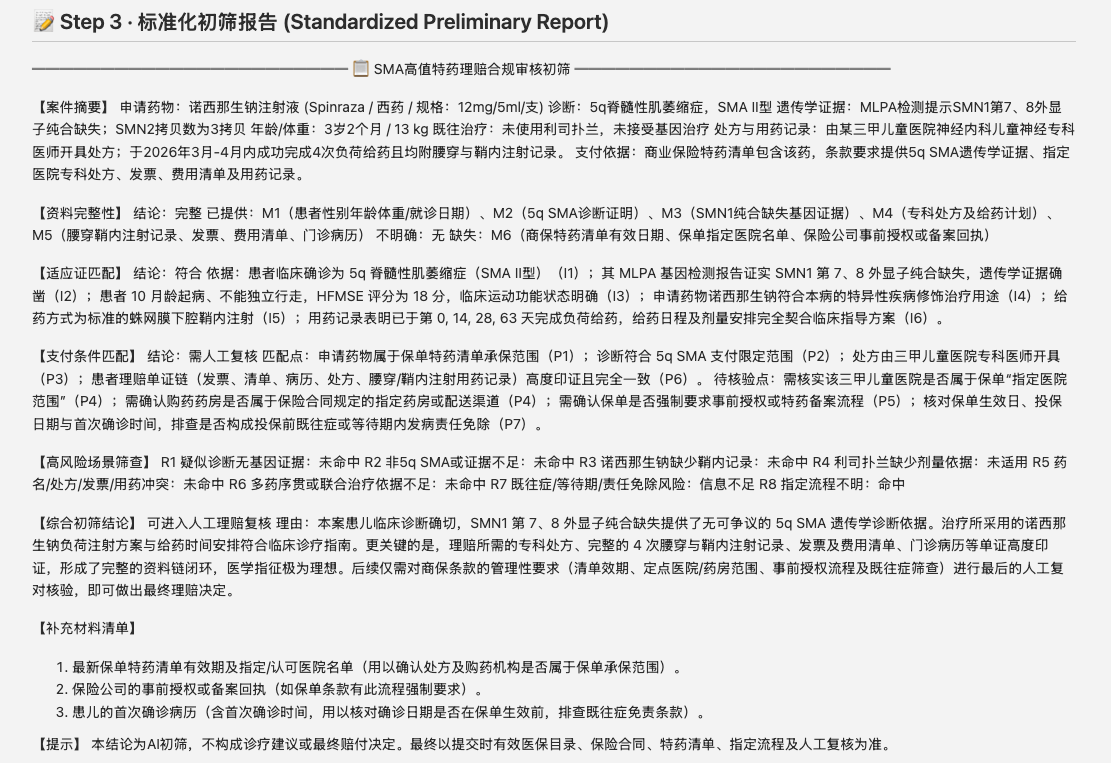
\includegraphics[width=0.92\textwidth]{images/Gemini-test-1.png}
\end{frame}

\subsection{跨模型差异分析与结论}
\begin{frame}[fragile]{跨模型差异分析模板}
  \small
  \begin{tabularx}{\textwidth}{>{\bfseries}l X}
    \toprule
    差异类型 & 分析口径 \\
    \midrule
    输出格式差异 & 是否严格按照Skill模板输出；是否漏掉资料完整性、适应证、支付条件或风险模块。 \\
    规则命中差异 & 是否漏判R规则，尤其是R3给药方式冲突、R6序贯治疗、R7等待期/既往症。 \\
    结论保守度差异 & 是否把“需人工复核”误写成“符合”或“可赔付”。 \\
    补充材料差异 & 是否提出关键补充材料，如基因检测、鞘内注射记录、医保结算单、授权备案。 \\
    合规边界差异 & 是否出现治疗建议、赔付承诺或对政策时效性的忽略。 \\
    \bottomrule
  \end{tabularx}
\end{frame}

\begin{frame}[fragile]{跨模型结果分析}
\small
\textbf{输出格式差异：}
DeepSeek与GPT均严格遵循Skill结构化模板，Gemini存在轻微模块压缩或重排，尤其在“支付条件”与“风险模块”表达上不够严格。

\vspace{0.2cm}
\textbf{规则命中差异：}
三类模型均能识别核心R规则（R3给药方式冲突、R6序贯治疗、R7等待期/既往症），但DeepSeek对规则触发更敏感，GPT次之，Gemini存在局部弱化。

\vspace{0.2cm}
\textbf{结论保守度差异：}
DeepSeek倾向“结构化拒绝/不符合”，GPT倾向“条件性不确定”，Gemini更易输出“可复核/建议补充材料”。

\vspace{0.2cm}
\textbf{补充材料差异：}
DeepSeek与GPT更稳定提出关键证据缺失（SMN1检测、鞘内注射记录等），Gemini补充材料提示更依赖语义生成而非规则触发。

\vspace{0.2cm}
\textbf{合规边界差异：}
DeepSeek合规边界最严格，基本不产生“隐含赔付倾向”；GPT较稳定；Gemini在部分案例中存在轻微治疗性表述扩展。
\end{frame}

\begin{frame}[fragile]{方法学限制}
\small
本实验结果存在潜在混杂因素，需谨慎解释模型间差异来源：
\begin{itemize}
  \item DeepSeek可能涉及中文输入后进行英文语义重编码，并在中英混合语义空间中完成Skill调用与推理，因此其“规则严格性”可能部分受到语言转换路径影响，而非纯规则执行能力差异。
  \item Gemini在部分样本中受限于Pro版本调用额度，有部分结果由3.1 Flash模型生成，该模型切换可能降低推理深度与约束执行强度，从而影响合规判定一致性。
  \item 因此，跨模型差异不仅来源于规则理解能力，还受到语言处理路径、模型版本切换与推理预算差异的共同影响。
\end{itemize}

\end{frame}

\begin{frame}[fragile]{跨模型验证结果的反思}
为提升Skill跨模型评估的可比性与稳定性，可在V2中强化以下机制：
\begin{itemize}
  \item 输出结构强约束：减少模型在医学解释层面的自由扩展
  \item 明确规则优先级：强化“缺失即否决/不可假设”的硬约束逻辑
  \item 引入风险分级与可解释评分体系：提升输出一致性与可量化程度
  \item 增加语言与模型路径控制机制：记录或限制多语言中介与模型切换带来的偏差
\end{itemize}

\end{frame}
